\renewcommand{\theequation}{\theenumi}
\begin{enumerate}[label=\thesection.\arabic*.,ref=\thesection.\theenumi]
\numberwithin{equation}{enumi}

%\renewcommand{\thefigure}{\theenumi.\arabic{figure}}
\begin{figure}[!ht]
\centering
\resizebox{\columnwidth}{!}{\input{./figs/triangle.tex}}
\caption{$\triangle ABC$ and $\triangle PQR$ by Latex-Tikz}
\label{fig:triangle_latex}	
\end{figure}
%
%
%\renewcommand{\thefigure}{\theenumi}
%
\item Since it is given that the triangles ABC and PQR have two sides and a median length equal, we have considered the following inputs for constructing the figures:
\\
%
\begin{table}[ht!]
\centering
\input{./tables/inp.tex}
\caption{To construct $\triangle $ ABC and $\triangle$ PQR}
\label{table:table1}	
\end{table}


\item The coordinates of the various points of triangle ABC in Fig. \ref{fig:triangle_latex} are:
%\label{}
\\
%
%\solution From the given information, 
%$\triangle ABC$ are 
\begin{align}
\vec{B} &= \myvec{0\\0} ,
\label{eq:constr_b}
\\
 \vec{C} &= \myvec{a\\0}, 
\label{eq:constr_c}
\end{align}

$\because \vec{M}$ is the midpoint of $BC$,
\begin{align}
\vec{M}= \frac{\vec{B}+\vec{C}}{2} =\myvec{a/2\\0},
\label{eq:constr_m}
\end{align}
Using the coordinates of $\vec{B}$ , $\vec{C}$ and input parameters, we can find the coordinates of vertex $\vec{A}$. 
The derived values are listed in  
Table. \ref{table:table2} 
\begin{table}[ht!]
\centering
\input{./tables/derived.tex}
\caption{To construct $\triangle $ ABC}
\label{table:table2}
\end{table}
%
\item Using the similar construction steps as triangle ABC, we can construct triangle PQR because they both have the same input parameters.
%
\\
\item To get the python code for Fig \ref{fig:triangle_python}, download it from
\begin{lstlisting}
codes/triangle_python.py
\end{lstlisting}
\begin{figure}[!ht]
\centering
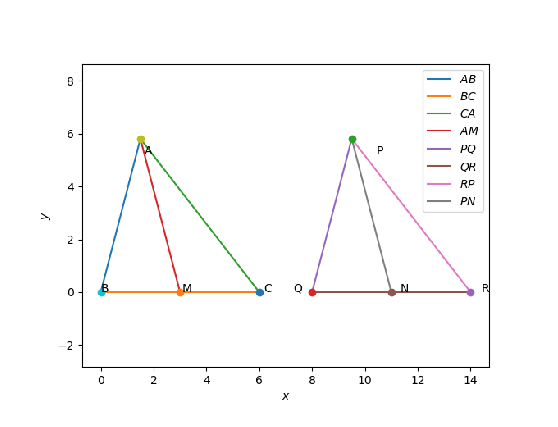
\includegraphics[width= \columnwidth]{Figure_1.eps}
\caption{$\triangle ABC$ and $\triangle PQR$ using Python}
\label{fig:triangle_python}
\end{figure}
%
and the equivalent latex-tikz code for Fig. \ref{fig:triangle_latex} from
\begin{lstlisting}
figs/triangle.tex
\end{lstlisting}
%
The above latex code can be compiled as a standalone document as
\begin{lstlisting}
figs/triangle_fig.tex
\end{lstlisting}



\end{enumerate}
